% !TEX root = ../intro-stellar-physics.tex

\section{The Coulomb barrier}

Let's take two nuclei with masses\sidenote{When doing kinematics, we shall make the approximation $m\approx A\mb$.} $A_{1}\mb$ and $A_{2}\mb$. This is a two-body problem, so we transform to the center-of-mass frame; the problem reduces to that of one particle, mass $A\mb = A_{1}A_{2}/(A_{1}+A_{2})\times\mb$, moving in a potential.  At distances $\gtrsim \val{2}{\fermi}$, the potential is all Coulomb\sidenote{We write the force between two electrons as $e^2/r^2$.},
\[ \frac{Z_{1}Z_{2}e^{2}}{r} = \val{1.44}{\MeV}\times Z_{1}Z_{2}\left(\frac{\val{1}{\fermi}}{r}\right). \]
We show in Fig.~\ref{f.tunneling} this Coulomb potential as a red curve.
At closer distances the nuclear potential forms a deep well with a repulsive core (blue curve in Fig.~\ref{f.tunneling}).

\begin{figure}[hb]
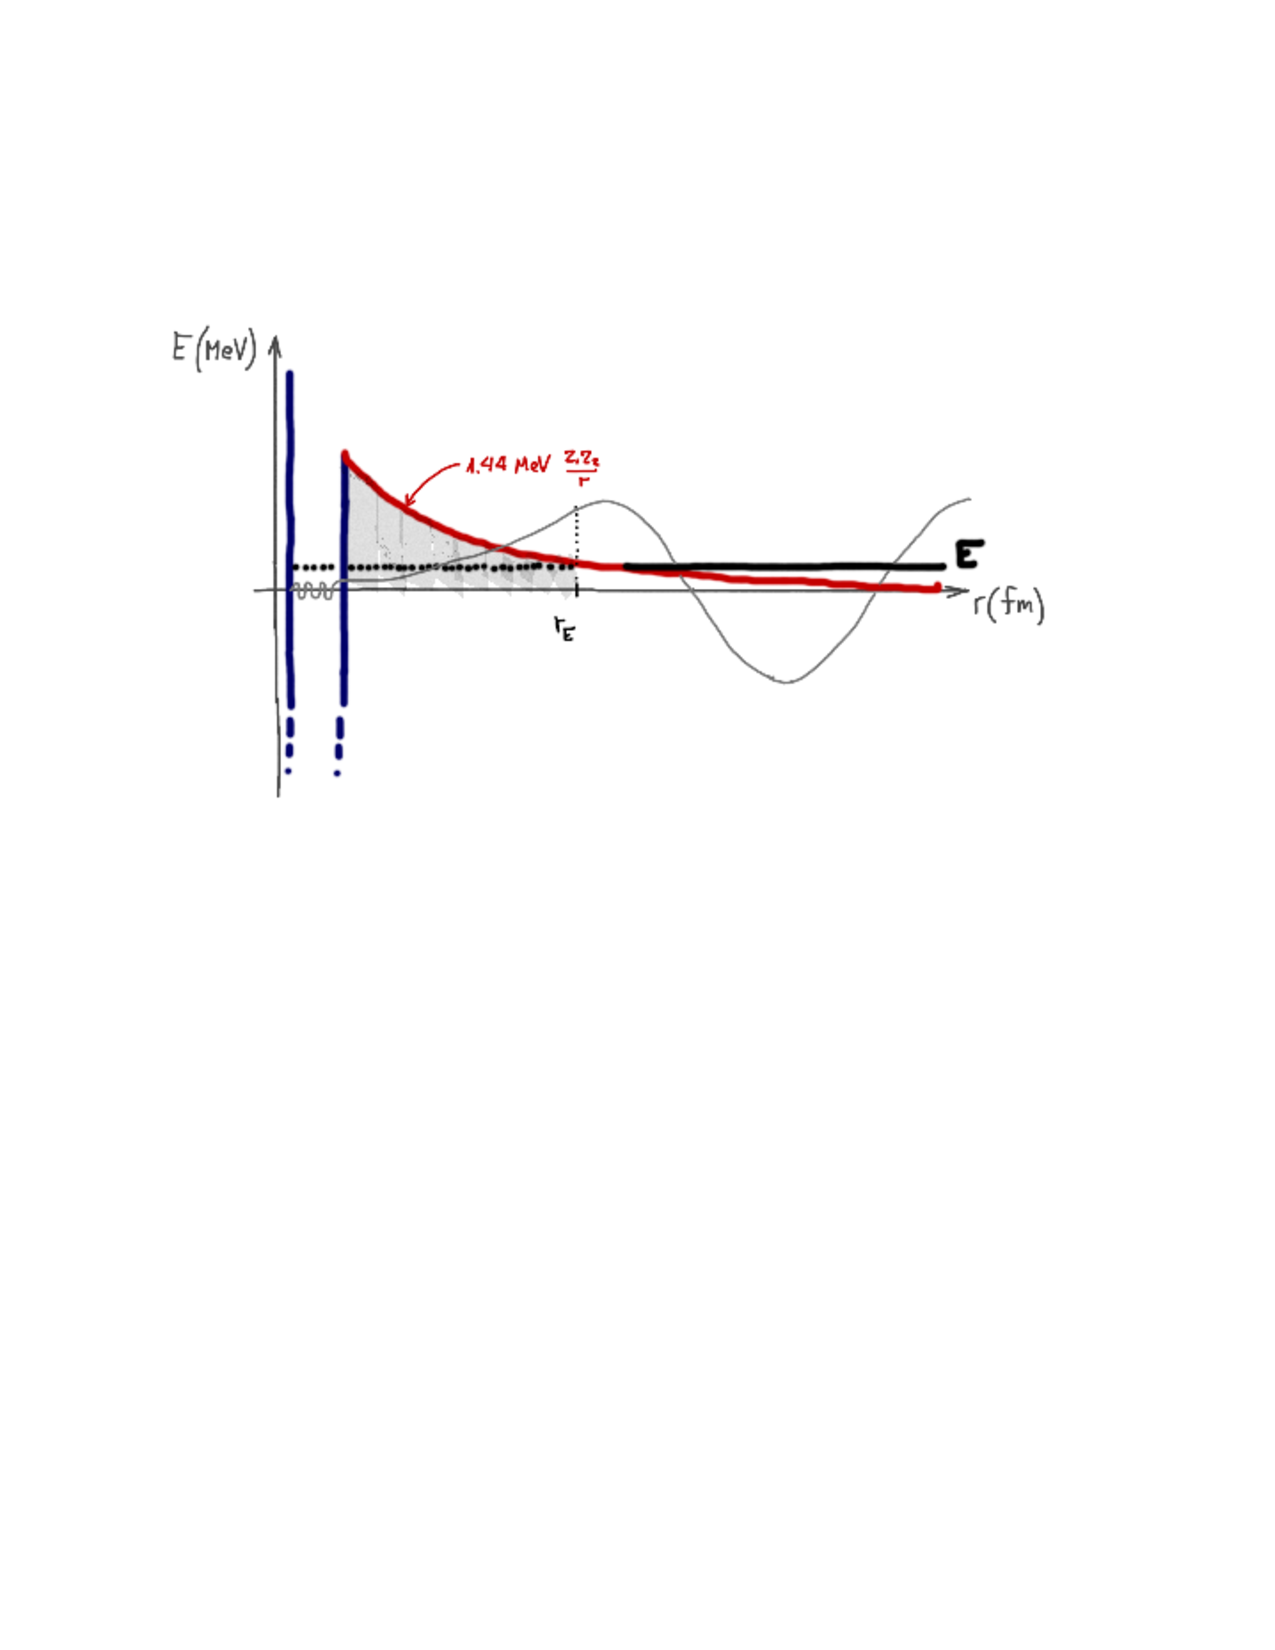
\includegraphics[width=\linewidth]{Tunneling}
\caption{Tunneling through the Coulomb potential barrier.}
\label{f.tunneling}
\end{figure}

\newthought{Suppose we shoot the particle in from infinity:} How close does the particle come before stopping? For the sun, $E \sim \val{1}{\keV}$ (black line in Fig.~\ref{f.tunneling}).  Equating this energy with the potential and solving for $r$ gives the \emph{turning radius}
\begin{equation}
	r_{E} = \frac{Z_{1}Z_{2}e^{2}}{E} = Z_{1}Z_{2}\times \left(\frac{\val{1}{\keV}}{E}\right) \times \val{1440}{\fermi}.
\end{equation}
This is much bigger than the nuclear radius.  Classically the particle can't go in the region $r<r_{E}$.

The world is quantum, however: the particle wavefunction (thin gray line) decreases exponentially in this region, but there is a finite probability for the particle to reach $r\sim\val{1}{\fermi}$.  This probability is
\[ \mathcal{P}\approx \exp\left[-2\pi^{2}\frac{r_{E}}{\lambda}\right] \]
where $\lambda = h/p$, $p$ being the momentum of the particle.

Expanding,
\[ \frac{2\pi^{2}r_{E}}{\lambda} = 2\pi^{2}\left(\frac{Z_{1}Z_{2}e^{2}}{E}\right)
	\left(\frac{p}{h}\right) = \left[\sqrt{2}\pi \frac{Z_{1}Z_{2}e^{2}}{\hbar}\right]\left(\frac{1}{E}\right)^{1/2}, \]
so we write
\begin{equation}
\mathcal{P} \approx \exp\left[-\left(\frac{\EG}{E}\right)^{1/2}\right],
\end{equation}
with
\[ \EG \equiv \textrm{``Gamow Energy''} = \left[\frac{2\pi^{2}Z_{1}Z_{2}e^{4}m}{\hbar^{2}}\right] = Z_{1}^{2}Z_{2}^{2}A \times \val{979}{\keV}.
\]

\section{The cross-section}
The cross-section for scattering in general is proportional to the ``size'' of the wavefunction, 
\[\sigma\propto \pi\left(\frac{\lambda}{2\pi}\right)^{2} = \pi \left(\frac{\hbar}{p}\right)^{2} = \pi\frac{\hbar^{2}}{2mE}.\]
To get the cross-section for a reaction, we multiply this by the probability of tunneling through the Coulomb barrier, $\mathcal{P} = \exp\left[-\left(\EG/E\right)^{1/2}\right]$, and a term $S(E)$ that accounts for the nuclear interaction.

Putting this all together, we write the reaction cross-section as
\begin{equation}\label{e.s-def}
\sigma(E) = \frac{S(E)}{E}\exp\left[-\left(\frac{\EG}{E}\right)\right].
\end{equation}
It turns out that $S(E)$ is nearly constant\sidenote{This is true as long as we are not close to a resonance---an energy level in the compound nucleus that matches the energy of the incoming particle.}, which helps with extrapolating the cross-section from laboratory energies  to the much lower stellar energies.

\section{The reaction rate}
Recall that the mean-free path of a particle is $\ell = (n\sigma)^{-1}$, where $n$ is the density of targets.  For a particle traveling at speed $v$, the mean time between collisions is therefore $\ell/v$; in a large ensemble of particles, this gives the mean rate, $r = n\sigma v$.  Here $v = |\bvec{v}_{1}-\bvec{v}_{2}|$ is the relative velocity between the particles.  Since the cross-section depends on energy, the rate at which any given particle 1 will react with particles of type 2 having velocities $\bvec{v}_{2}$ in a range $\dif^{3}v_{2}$ is
\[ n_{2} \sigma |\bvec{v}_{1}-\bvec{v}_{2}| \left(\frac{m_{2}}{2\pi kT}\right)^{3/2}\exp\left(-\frac{m_{2}v_{2}^{2}}{2kT}\right) \,\dif^{3}v_{2}. \]
The extra terms are because the particles have a Maxwell-Boltzmann distribution of velocities.  To get the total rate per unit volume, we then have to multiply by the number of particles of type 1 having velocities $\bvec{v}_{1}$ in a range $\dif^{3} v_{1}$ and integrate\sidenote{If particle 1 and particle 2 are identical, for example in the reaction $p+p$, then divide the rate by 2 to avoid double-counting.} over $\dif^{3}v_{1}\,\dif^{3}v_{2}$:
\begin{eqnarray}\label{e.rate-joint}
\lefteqn{r_{12} = n_{1}n_{2}  \left[\frac{m_{1}m_{2}}{(2\pi kT)^{2}}\right]^{3/2}}
  \nonumber\\ &&\times\int\! \sigma(E) v\exp\left(-\frac{m_{1}v_{1}^{2}}{2kT}-\frac{m_{2}v_{2}^{2}}{2kT}\right)  \,\dif^{3} v_{1}\,\dif^{3}v_{2}.
\end{eqnarray}
Now $E$ and $v$ are the relative energies and velocity in the center-of-mass frame.  We can change variable using the relations
\begin{eqnarray*}
\bvec{v}_{1} &=& \bvec{V} - \frac{m_{2}}{m_{1}+m_{2}} \bvec{v}\\
\bvec{v}_{2} &=& \bvec{V} + \frac{m_{1}}{m_{1}+m_{2}} \bvec{v}.
\end{eqnarray*}
where $V$ is the center-of-mass velocity. It is straightforward to show that $\dif v_{1,x}\,\dif v_{2,x} = \dif V_{x}\dif v_{x}$, and likewise for the $y,z$ directions.  Furthermore, $m_{1}v_{1}^{2} + m_{2}v_{2}^{2} = (m_{1}+m_{2})V^{2} + m v^{2}$, and multiplying and dividing the integral in equation~(\ref{e.rate-joint}) by $m_{1}+m_{2}$ allows us to write
\begin{eqnarray*}
\lefteqn{r_{12} = n_{1}n_{2} \left(\frac{m_{1}+m_{2}}{2kT}\right)^{3/2}\left(\frac{m}{2kT}\right)^{3/2}}\\
&&\times \int\!\dif^{3}V \int\!\dif^{3}v \,\sigma(E)v \exp\left[-\frac{mv^{2}}{2kT}\right]
 \exp\left[-\frac{(m_{1}+m_{2})V^{2}}{2kT}\right].
\end{eqnarray*}
The integral over $\dif^{3}V$ can be factored out and is normalized to unity. Hence we have for the reaction rate between a pair of particles 1 and 2, 
\begin{eqnarray}\label{e.rate}
r_{12} &=& n_{1}n_{2}\left\{\left(\frac{m}{2\pi kT}\right)^{3/2}\int_{0}^{\infty}\! \sigma(E) v \exp\left(-\frac{mv^{2}}{2kT}\right)  4\pi v^{2}\,\dif v\right\}.\nonumber\\
 &\equiv& \frac{1}{1+\delta_{12}}n_{1}n_{2}\langle\sigma v\rangle.
\end{eqnarray}
The term in $\{\}$ is the averaging over the joint distribution of the cross-section times the velocity, and is usually denoted as $\langle\sigma v\rangle$. 

Changing variables to $E = mv^{2}/2$ in equation~(\ref{e.rate}) and inserting the formula for the cross-section, equation~(\ref{e.s-def}), gives
\begin{equation}\label{e.integral}
\langle\sigma v\rangle = \left(\frac{8}{\pi m}\right)^{1/2}\left(\frac{1}{kT}\right)^{3/2}\int_{0}^{\infty}\!S(E)\exp\left[-\left(\frac{\EG}{E}\right)^{1/2}-\frac{E}{kT}\right]\,\dif E.
\end{equation}
Now, we've assumed that $S(E)$ varies slowly; but look at the argument of the exponential. This is a competition between a rapidly rising term $\exp[-(\EG/E)^{1/2}]$ and a rapidly falling term $\exp(-E/kT)$. As a result, the exponential will have a strong peak, and we can expand the integrand in a Taylor series about the maximum. Let 
\[
f(E) = -\left(\frac{\EG}{E}\right)^{1/2} - \frac{E}{kT}.
\]
Then we can write 
\begin{eqnarray*}
\lefteqn{\int_{0}^{\infty}\!S(E)\exp\left[-\left(\frac{\EG}{E}\right)^{1/2}-\frac{E}{kT}\right]\,\dif E}\\
&\approx&
	\int_{0}^{\infty}\! S(\Epk)\exp\left[f(\Epk) + \frac{1}{2}\left.\frac{\dif^{2} f}{\dif E^{2}}\right|_{E=\Epk}\left(E-\Epk\right)^{2}\right].
\end{eqnarray*}
Here $\Epk$ is found by solving $(\dif f/\dif E)|_{E=\Epk} = 0$. This trick allows us to turn the integral into a Gaussian! (Before the internet, all there was to do for fun were integrals.)

Solving for \Epk, we get
\[
\Epk = \frac{\EG^{1/3}(kT)^{2/3}}{2^{2/3}},
\]
and 
\[ \exp\left[f(\Epk)\right] = \exp\left[-3\left(\frac{\EG}{4kT}\right)^{1/3}\right].
\]
Further,
\[
\left.\frac{1}{2}\frac{\dif^{2}f}{\dif E^{2}}\right|_{E=\Epk} = -\frac{3}{2(2\EG)^{1/3}(kT)^{5/3}} = -\frac{3}{4\Epk kT}.
\]
Defining a variable $\Delta = 4(\Epk kT/3)^{1/2}$, our integral becomes
\begin{eqnarray}\label{e.integral2}
\lefteqn{\langle\sigma v\rangle = \left(\frac{8}{\pi m}\right)^{1/2}\left(\frac{1}{kT}\right)^{3/2}}\nonumber\\
&&\times S(\Epk)
  \exp\left[-3\left(\frac{\EG}{4kT}\right)^{1/3}\right]
  \int_{0}^{\infty}\!\exp\left[-\frac{(E-\Epk)^{2}}{(\Delta/2)^{2}}\right]\,\dif E.
\end{eqnarray}
How well does this approximation do?  Figure~\ref{f.integrand} shows the integrand (\emph{solid line}) and the approximation by a Gaussian (\emph{dashed line}).  Although the integrand is skewed to the right, the area is approximately the same.  
\begin{marginfigure}[-16\baselineskip]
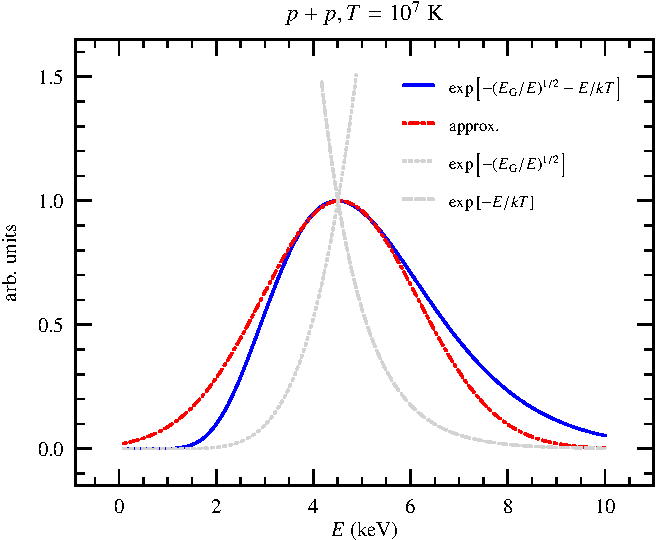
\includegraphics[width=\linewidth]{coulomb_integrand}
\caption[Terms in integrand for calculating Coulomb barrier]{Integrand of eq.~(\protect\ref{e.integral}) (\emph{solid line}) and the Gaussian (\emph{dot-dashed line}) constructed by expanding to second order the argument of the exponential. The parameters for $\EG$ were taken from the $p+p$ reactions ($Z_{1}Z_{2}=1$, $A = 1/2$), and the temperature is $\val{10^{7}}{\K}$.  Note that the grey curves, showing the two terms of the exponential, have been rescaled to fit on the same plot.}
\label{f.integrand}
\end{marginfigure}

Another simplification can be made because both the Gaussian and the original integrand go to zero as $E\to 0$.  As a result, we can extend the lower bound of our integral (eq.~[\ref{e.integral2}]) to $-\infty$, and obtain
\begin{eqnarray}\label{e.rate2}
\langle\sigma v\rangle &\approx& \left(\frac{8}{\pi m}\right)^{1/2}\left(\frac{1}{kT}\right)^{3/2} S(\Epk) \exp\left[-3\left(\frac{\EG}{4kT}\right)^{1/3}\right]\frac{\Delta}{2}\nonumber\\
 &=& \frac{2^{13/6}}{\sqrt{3m}}\frac{\EG^{1/6}}{(kT)^{2/3}} \exp\left[-3\left(\frac{\EG}{4kT}\right)^{1/3}\right]  S(\Epk).
\end{eqnarray}
On to some numbers. Table~\ref{t.reaction} lists quantities for some common reactions. A couple of notes. First, $\Delta/\Epk$ indicates how well our Gaussian approximation works---you will see it is less than 1 in all cases. We evaluated $\Delta/\Epk$, which decreases with temperature as $T^{-1/6}$, at $T = \val{10^{7}}{\K}$. Second, the quantity $n(T)$ is the exponent if we want to approximate the reaction rate as a power-law, $r\propto T^{n}$.  We compute this as 
\begin{equation}\label{e.exponent}
 n(T) = \dd{\ln r}{\ln T} = -\frac{2}{3} + \left(\frac{\EG}{4kT}\right)^{1/3},
\end{equation}
as you can verify for yourself. In the table, the exponent is evaluated at $T = \val{10^{7}}{\K}$; the exponent $n$ depends on temperature. Finally, note the size of $\EG/(4k)$.  This makes the argument of the exponential in equation~(\ref{e.rate2}) large in absolute value, and sets the temperature scale at which a given reaction comes into play.
 
\begin{table}[hb]
\caption{\label{t.reaction} Parameters for non-resonant reactions}
\begin{center}
\begin{tabular}{lrrrrrr}
\hline
Reaction & $p+p$ & $p+\helium[3]$ & $\helium[3]+\helium[3]$ & $p+\lithium[7]$ & $p+\carbon$\\
\hline\hline
$A$ & 1/2 & 3/4 & 3/2 & 0.88 & 0.92 \\
$Z_{1}Z_{2}$ & 1 & 2 & 4 & 3 & 6 \\
$\EG$ (MeV) & 0.489 & $2.94$ & $23.5$ & $7.70$ & $32.5$\\
$\EG/(4k)$ (GK) & $1.4$ & $8.5$ & $68.0$ & $22.0$ & $94.0$ \\
$\Epk|_{T=\val{10^{7}}{\K}}$ (keV) & 4.5 & 8.2 & 16.3 & 11.3 & 18.2\\
$\Delta/\Epk|_{T=\val{10^{7}}{\K}}$ & 1.0 & 0.75 & 0.53 & 0.64 & 0.50 \\
$n(T = \val{10^{7}}{\K})$ & 4.6 & 8.8 & 18.3 & 12.4 & 20.5\\
\hline
\end{tabular}
\end{center}
\end{table}
